\section{Vertex Shader}

\subsection{Overview}
\begin{frame}{Vertex Shader Stage}
  \small
  \begin{columns}
    \begin{column}{0.6\textwidth}
      \begin{raybox}{Vertex Shader}
        \textbf{Input:} Individual vertices with attributes \\
        \textbf{Output:} Transformed vertices in clip space

        \vspace{0.3cm}
        \textbf{Purpose:}
        \begin{itemize}
          \item Transform vertex positions through coordinate spaces
          \item Calculate per-vertex lighting (Gouraud shading)
          \item Pass attributes to next stage
          \item Apply animations and deformations
        \end{itemize}

        \vspace{0.2cm}
        \textcolor{PrimaryColor}{\textbf{Programmable stage - you write the code!}}
      \end{raybox}
    \end{column}
    \begin{column}{0.4\textwidth}
      \begin{tikzpicture}[scale=0.7]
        % Input vertex
        \node[circle, draw, fill=ObjectColor!20, minimum size=0.8cm] (input) at (0,3) {
          \tiny
          \begin{minipage}{0.6cm}
            \centering
            Vertex \\
            (Model)
          \end{minipage}
        };

        % Vertex Shader box
        \node[rectangle, draw, fill=PrimaryColor!30, minimum width=2cm, minimum height=1.2cm] (vs) at (0,1.5) {
          \begin{minipage}{1.8cm}
            \centering
            \textbf{Vertex} \\
            \textbf{Shader}
          \end{minipage}
        };

        % Output vertex
        \node[circle, draw, fill=SecondaryColor!20, minimum size=0.8cm] (output) at (0,0) {
          \tiny
          \begin{minipage}{0.6cm}
            \centering
            Vertex \\
            (Clip)
          \end{minipage}
        };

        \draw[->, thick] (input) -- (vs);
        \draw[->, thick] (vs) -- (output);

        % Side annotations
        \node[right] at (1,3) {\scriptsize Position, Normal, UV, ...};
        \node[right] at (1,0) {\scriptsize \texttt{gl\_Position}, attributes};
      \end{tikzpicture}
    \end{column}
  \end{columns}
\end{frame}

\subsection{Coordinate Space Transformations}
\begin{frame}{The Transformation Pipeline}
  \begin{center}
    \begin{tikzpicture}[scale=0.8]
      % Model Space
      \node[rectangle, draw, fill=ObjectColor!20, minimum width=1.8cm, minimum height=0.8cm] (model) at (0,4) {
        \begin{minipage}{1.6cm}
          \centering
          \textbf{Model} \\
          \textbf{Space}
        \end{minipage}
      };

      % World Space
      \node[rectangle, draw, fill=PrimaryColor!20, minimum width=1.8cm, minimum height=0.8cm] (world) at (3,4) {
        \begin{minipage}{1.6cm}
          \centering
          \textbf{World} \\
          \textbf{Space}
        \end{minipage}
      };

      % View Space
      \node[rectangle, draw, fill=SecondaryColor!20, minimum width=1.8cm, minimum height=0.8cm] (view) at (6,4) {
        \begin{minipage}{1.6cm}
          \centering
          \textbf{View} \\
          \textbf{Space}
        \end{minipage}
      };

      % Clip Space
      \node[rectangle, draw, fill=AccentColor!20, minimum width=1.8cm, minimum height=0.8cm] (clip) at (9,4) {
        \begin{minipage}{1.6cm}
          \centering
          \textbf{Clip} \\
          \textbf{Space}
        \end{minipage}
      };

      % NDC
      \node[rectangle, draw, fill=LightGray, minimum width=1.8cm, minimum height=0.8cm] (ndc) at (6,2) {
        \begin{minipage}{1.6cm}
          \centering
          \textbf{NDC} \\
          \textbf{Space}
        \end{minipage}
      };

      % Screen Space
      \node[rectangle, draw, fill=RayColor!20, minimum width=1.8cm, minimum height=0.8cm] (screen) at (3,2) {
        \begin{minipage}{1.6cm}
          \centering
          \textbf{Screen} \\
          \textbf{Space}
        \end{minipage}
      };

      % Arrows with matrix labels
      \draw[->, thick] (model) -- (world);
      \node[above] at (1.5,4.2) {\scriptsize Model Matrix};

      \draw[->, thick] (world) -- (view);
      \node[above] at (4.5,4.2) {\scriptsize View Matrix};

      \draw[->, thick] (view) -- (clip);
      \node[above] at (7.5,4.2) {\scriptsize Projection Matrix};

      \draw[->, thick] (clip) -- (ndc);
      \node[right] at (9.2,3) {\scriptsize Perspective Divide};

      \draw[->, thick] (ndc) -- (screen);
      \node[below] at (4.5,1.8) {\scriptsize Viewport Transform};

      % Vertex shader boundary
      \draw[dashed, PrimaryColor, thick, rounded corners] (-0.5,3.3) rectangle (9.5,4.7);
      \node[below right] at (-0.5,3.3) {\textcolor{PrimaryColor}{\textbf{Vertex Shader}}};

      % Hardware boundary
      \draw[dashed, DarkGray, thick, rounded corners] (5.5,1.3) rectangle (9.5,2.7);
      \node[below right] at (5.5,1.3) {\textcolor{DarkGray}{\textbf{Hardware}}};
    \end{tikzpicture}
  \end{center}
\end{frame}

\begin{frame}{Transformation Matrices}
  \only<1>{
    \begin{columns}
      \begin{column}{0.5\textwidth}
        \begin{mathbox}{Model Matrix}
          \textbf{Purpose:} Object-to-world transformation
          \begin{align*}
            \mathbf{M} &= \mathbf{T} \cdot \mathbf{R} \cdot \mathbf{S}
          \end{align*}

          \begin{itemize}
            \item \textbf{T}: Translation
            \item \textbf{R}: Rotation
            \item \textbf{S}: Scale
          \end{itemize}

          \vspace{0.2cm}
          Transforms from model's local coordinates to world coordinates.
        \end{mathbox}
      \end{column}
      \begin{column}{0.5\textwidth}
        \begin{conceptbox}{View Matrix}
          \textbf{Purpose:} World-to-camera transformation
          \begin{align*}
            \mathbf{V} &= \text{lookAt}(\mathbf{eye}, \mathbf{target}, \mathbf{up})
          \end{align*}

          Transforms from world coordinates to camera/eye coordinates.

          \vspace{0.2cm}
          Camera is at origin, looking down -Z axis.
        \end{conceptbox}
      \end{column}
    \end{columns}
  }
  \only<2>{
    \begin{mathbox}{Projection Matrix}
      \textbf{Purpose:} Camera-to-clip space transformation

      \textbf{Perspective:}
      \begin{align*}
        \mathbf{P}_{\text{persp}} &=
        \begin{pmatrix}
          \frac{1}{\tan(\text{fov}/2) \cdot \text{aspect}} & 0 & 0 & 0 \\
          0 & \frac{1}{\tan(\text{fov}/2)} & 0 & 0 \\
          0 & 0 & \frac{f+n}{n-f} & \frac{2fn}{n-f} \\
          0 & 0 & -1 & 0
        \end{pmatrix}
      \end{align*}
      \textbf{Orthographic:}
      \begin{align*}
        \mathbf{P}_{\text{ortho}} &=
        \begin{pmatrix}
          \frac{2}{r-l} & 0 & 0 & -\frac{r+l}{r-l} \\
          0 & \frac{2}{t-b} & 0 & -\frac{t+b}{t-b} \\
          0 & 0 & \frac{-2}{f-n} & -\frac{f+n}{f-n} \\
          0 & 0 & 0 & 1
        \end{pmatrix}
      \end{align*}
    \end{mathbox}
  }
\end{frame}

\begin{frame}[fragile]{Vertex Shader Example}
  \begin{columns}
    \begin{column}{0.6\textwidth}
      \begin{minted}[fontsize=\scriptsize, bgcolor=LightGray!20]{glsl}
#version 330 core
// Vertex shader inputs
layout (location = 0) in vec3 aPos;
layout (location = 1) in vec3 aNormal;
layout (location = 2) in vec2 aTexCoord;
// Outputs to fragment shader
out vec3 FragPos;
out vec3 Normal;
out vec2 TexCoord;
// Uniform variables
uniform mat4 model;
uniform mat4 view;
uniform mat4 projection;

void main() {
    FragPos = vec3(model * vec4(aPos, 1.0));
    Normal = mat3(transpose(inverse(model)))
              * aNormal;
    TexCoord = aTexCoord;

    gl_Position = projection
                  * view
                  * vec4(FragPos, 1.0);
}
      \end{minted}
    \end{column}
    \begin{column}{0.4\textwidth}
      \begin{conceptbox}{Output Variables}
        \texttt{\textcolor{PrimaryColor}{gl\_Position}} - \\ Clip space position
      \end{conceptbox}
    \end{column}
  \end{columns}
\end{frame}

\subsection{Vertex-Level Shading}
\begin{frame}{Gouraud Shading}
  \begin{columns}
    \begin{column}{0.6\textwidth}
      \begin{raybox}{Gouraud (Per-Vertex) Shading}
        Compute lighting at vertices, interpolate across triangles

        \vspace{0.3cm}
        \textbf{Process:}
        \begin{enumerate}
          \item Calculate lighting at each vertex
          \item Output vertex color
          \item Hardware interpolates colors across triangle
        \end{enumerate}

        \vspace{0.3cm}
        \textbf{Pros:} Fast, good for distant objects \\
        \textbf{Cons:} Poor specular highlights, faceted appearance
      \end{raybox}
    \end{column}
    \begin{column}{0.4\textwidth}
      \begin{tikzpicture}[scale=0.6]
        % Triangle with vertex normals
        \coordinate (A) at (0,0);
        \coordinate (B) at (3,0);
        \coordinate (C) at (1.5,2.5);

        % Draw triangle
        \draw[thick, ObjectColor] (A) -- (B) -- (C) -- cycle;

        % Vertex points
        \fill[PrimaryColor] (A) circle (3pt);
        \fill[SecondaryColor] (B) circle (3pt);
        \fill[AccentColor] (C) circle (3pt);

        % Normal vectors
        \draw[->, thick, PrimaryColor] (A) -- ++(210:0.8);
        \draw[->, thick, SecondaryColor] (B) -- ++(330:0.8);
        \draw[->, thick, AccentColor] (C) -- ++(90:0.8);

        % Light source
        \node[circle, fill=LightColor, minimum size=0.4cm] (light) at (-1,3) {\tiny \faIcon{lightbulb}};
        \draw[dashed, LightColor] (light) -- (A);
        \draw[dashed, LightColor] (light) -- (B);
        \draw[dashed, LightColor] (light) -- (C);

      \end{tikzpicture}

      \vspace{0.5cm}

      \begin{center}
        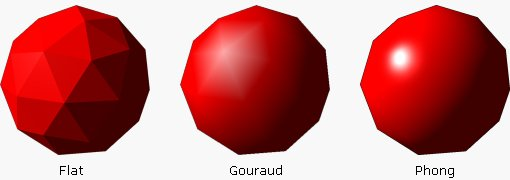
\includegraphics[width=\textwidth]{images/shading.jpg}
      \end{center}
    \end{column}
  \end{columns}
\end{frame}